% Results

Autoencoder networks generate compressed representations of data by propagating inputs through \textit{dimension bottlenecks}, wherein high-dimensional inputs are compressed to lower-dimensional representations.
The intensity of the dimension bottleneck imposed by an autoencoder is encapsulated by its \textit{compression ratio} --- that is, the ratio between the number of nodes in the input layer, and the number of nodes in the smallest hidden layer.
In particular, the greater the intensity of dimension bottleneck, the greater the quantity of data that must be discarded to produce low-dimension representations, and the greater the consequent degradation in data-accuracy of reconstructed inputs.
Demonstrating this notion, Figures \ref{fig:decoded-instances} and \ref{fig:decoded-instances-bias} present example image reconstructions for networks of varying compression ratios.
While low compression ratios (such as 7x and 14x) produce highly legible reconstructions of the original handwritten images, reconstruction accuracy diminishes drastically as compression ratios increase beyond 14x, likely as a reflection of the quantity of data that must be discarded to produce such highly compressed repreesntations.

Formally, the present analysis documents monotonically increasing reconstruction error in response to increasing compression ratios imposed by autoencoder networks (Table \ref{table:mse-final}, Figure \ref{fig:training-loss}).
In both cases of inclusion and exclusion of bias units, the most accurate reconstruction of input images was achieved by networks with  114 hidden nodes, and the least drastic compression ratios (MSE of 0.0085 and 0.0138 with and without inclusion of bias units respectively). 
While doubling compression ratios from 7x to 14x only resulted in minor degradation in reconstruction accuracy (MSE of 0.0160 and 0.0208 with and without inclusion of bias units respectively), compression ratios beyond 14x were associated with markedly higher reconstruction error compared to best observed performance.

Notably, however, average reconstruction error across the validation dataset masks substantial heterogeneity in model performance with respect to particular data subclasses.
Figure \ref{fig:mse-by-class} shows mean-squared error disaggregated by annotated label of instances processed by autoencoder networks.
Between-class differences in MSE suggest that estimated autoencoder networks exhibit varied proficiency in reconstructing particular digits. 
Specifically, digits with simple, linear structures --- such as 1s and 7s --- are more accurately reconstructed from compressed representations by all models, in comparison to digits with complex, curved structures -- such as 3s, 6s, and 8s. 

Unlike the effect of compression ratios, the inclusion of bias units within network architectures elicited mixed changes in reconstruction performance.
Firstly, reconstruction accuracies for networks with high compression ratios (392x and 196x) were relatively unaffected by  inclusion or exclusion of bias units (Table \ref{table:mse-final}, Figure \ref{fig:training-loss}).
Secondly, while architectures with lower compression ratios exhibited noticeable differences in reconstruction accuracy when implemented with and without bias units, the direction of these differences were inconsistent across the range of estimated models.
Such inconsistencies in the direction of affect resulting from imposition bias units are more likely an artefact of the stochastic nature of model training, rather than indicative of true reconstruction performance of underlying architectures. 

\begin{figure}
    \caption{Reconstructed instances disaggregated by compression ratio (no bias units)}
	\label{fig:decoded-instances}
	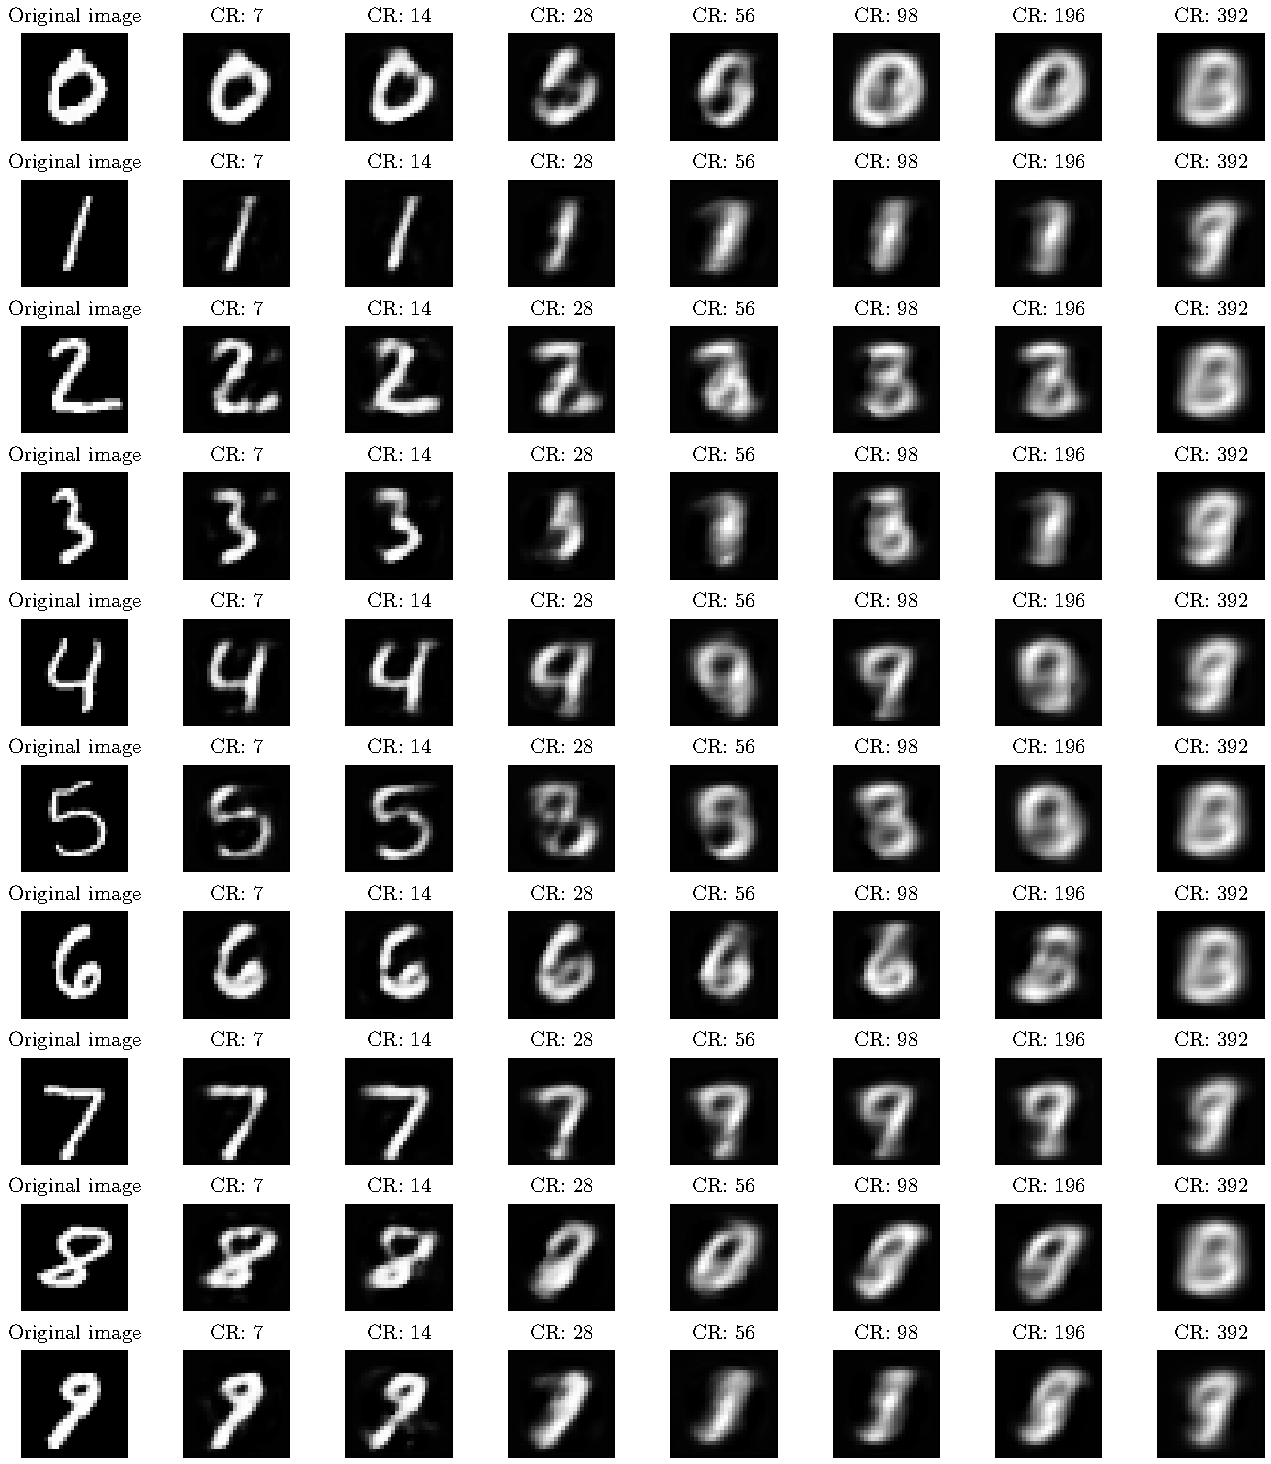
\includegraphics[width=1.0\textwidth]{graphics/decoded_instances.pdf}
    \textbf{Notes}: Reconstructed images are generated by encoding and decoding a stimulus image using a trained autoencoder networks with varying hidden layers, and bias set to zero. Columns separate reconstructed images by compression ratio (CR). Rows separate reconstructed images by the input stimulus (uncompressed) image. The first entry in each row is the stimulus image used to generate the following reconstructions.
\end{figure}

\begin{figure}
    \caption{Reconstructed instances disaggregated by compression ratio (including bias units)}
	\label{fig:decoded-instances-bias}
	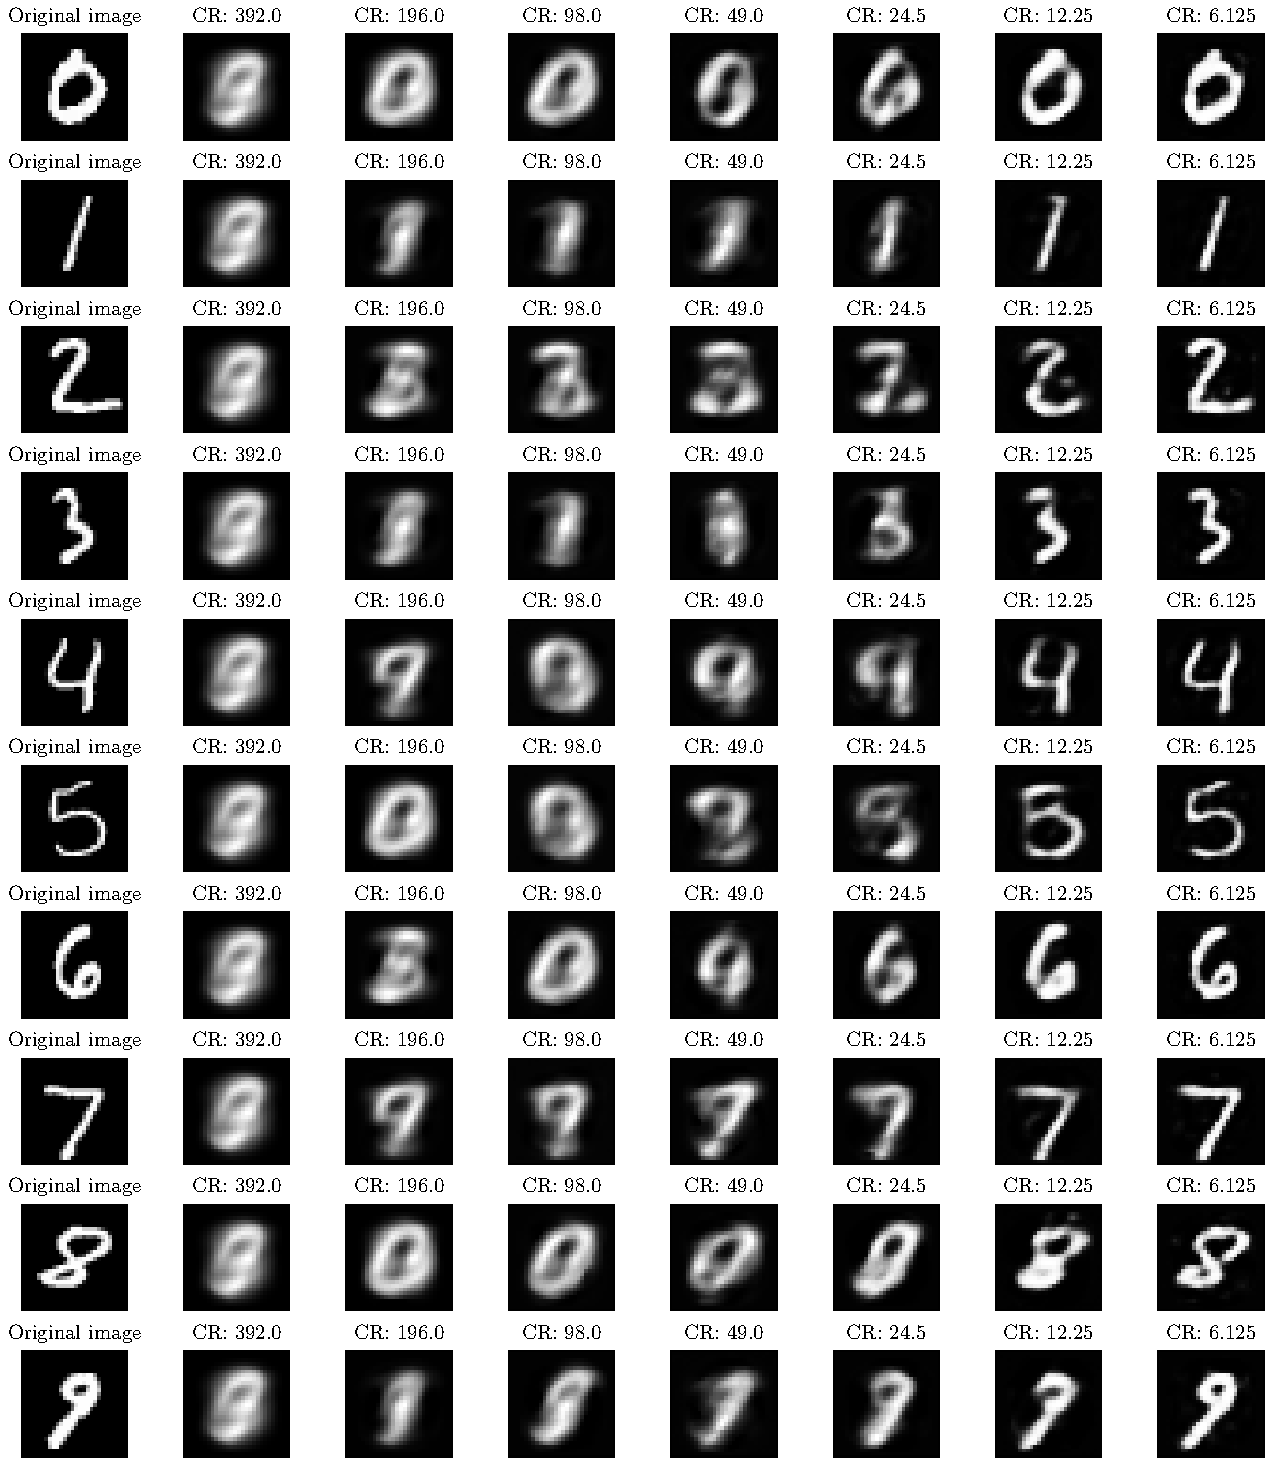
\includegraphics[width=1.0\textwidth]{graphics/decoded_instances_bias.pdf}
    \textbf{Notes}: Reconstructed images are generated by encoding and decoding a stimulus image using a trained autoencoder networks with varying hidden layers, and bias units included. Columns separate reconstructed images by compression ratio (CR). Rows separate reconstructed images by the input stimulus (uncompressed) image. The first entry in each row is the stimulus image used to generate the following reconstructions.
\end{figure}

\begin{figure}
    \caption{Mean-squared error (MSE) for reconstructed images disaggregated by MNIST class}
	\label{fig:mse-by-class}
	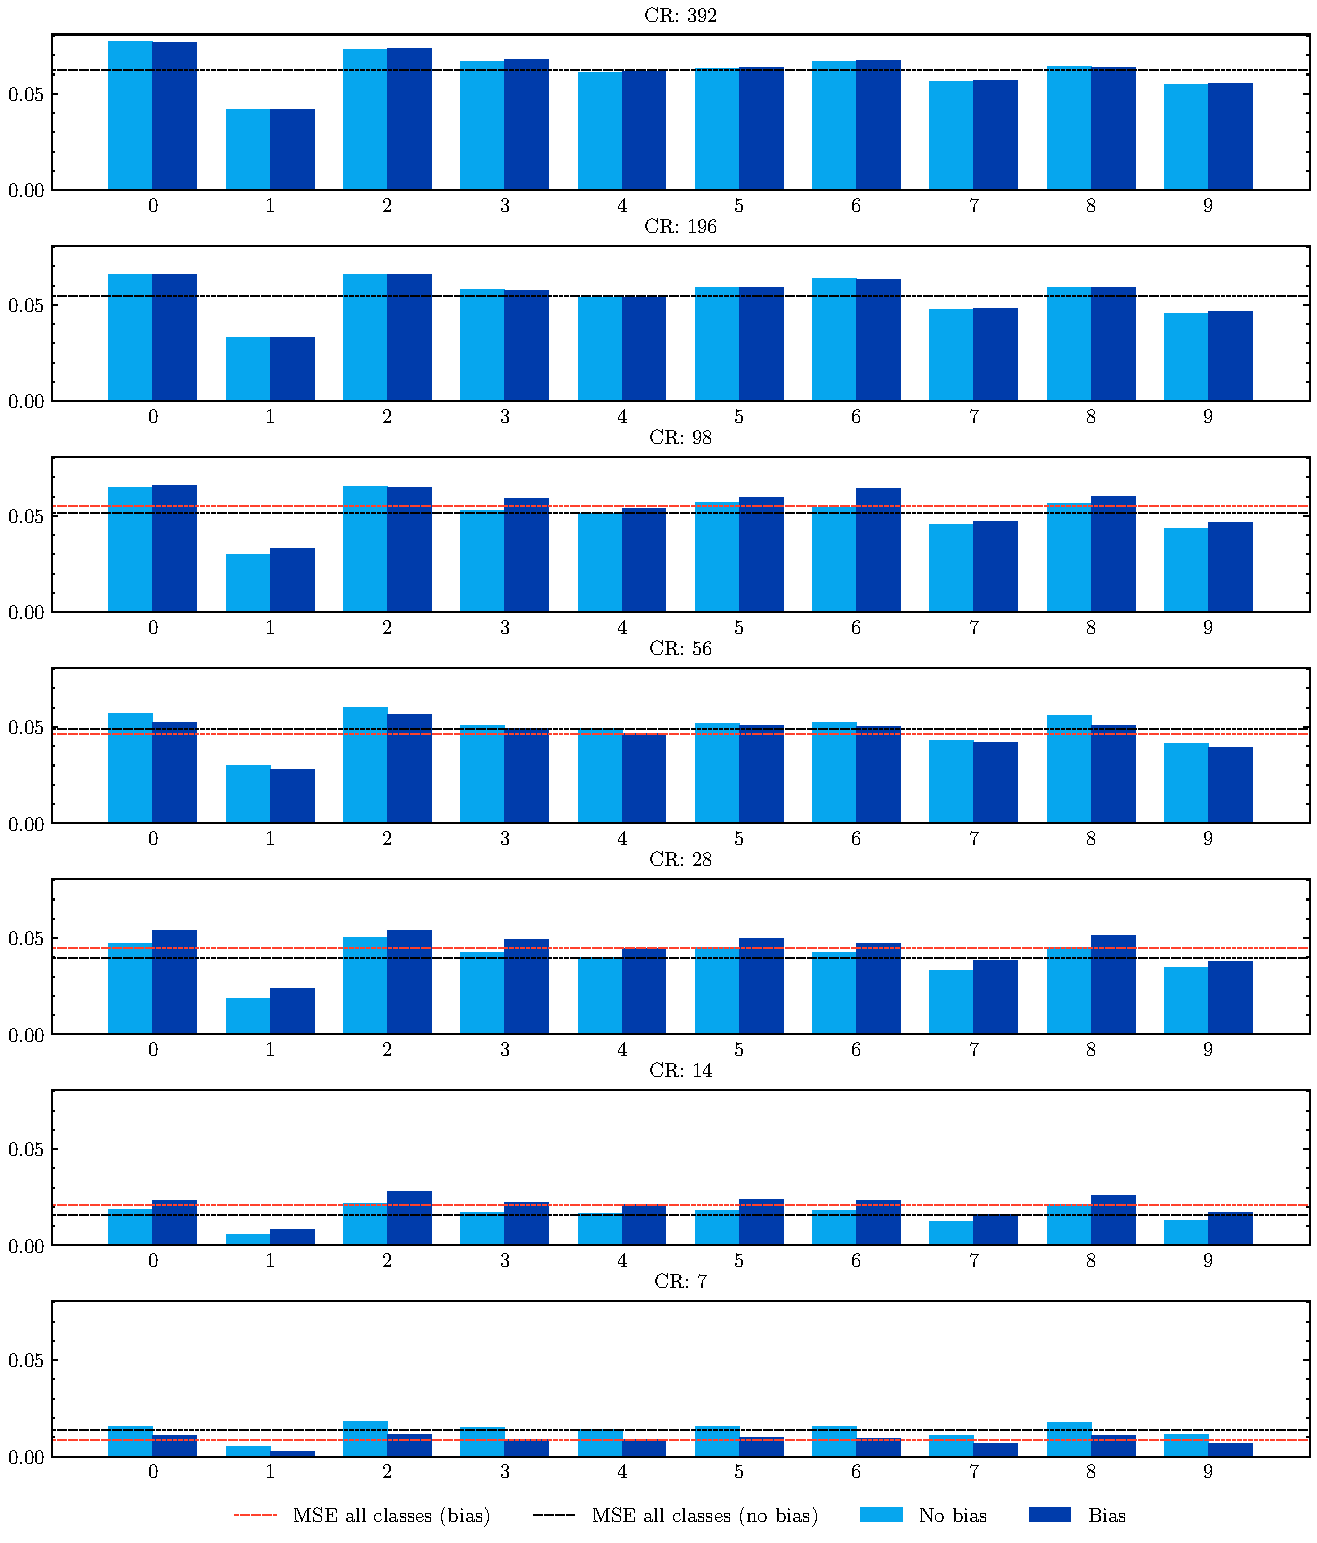
\includegraphics[width=1.0\textwidth]{graphics/mse_by_class.pdf}
    \textbf{Notes}: Mean squared error (MSE) across validation partition of MNIST dataset (N=10,000), disaggregated by annotated class of image instance. MSE is calculated after training models for 50 epochs. Autoencoder network architectures are split by compression ratio (CR), and inclusion of bias units.
\end{figure}


\begin{table}[h]
	\caption{Mean-squared error (MSE) for reconstructed images \label{table:mse-final}}
	\centering
	\begin{tabular}{lrrrr}
		\toprule
			Model &  MSE  \\
		\midrule
			\addlinespace{}
			\parbox{12.5cm}{Compression ratio: 392} & 0.0621 \\
			\addlinespace{}
			Compression ratio: 392 (bias) 	& 0.0624 \\
			\addlinespace{}
			Compression ratio: 196 			& 0.0547 \\
			\addlinespace{}
			Compression ratio: 196 (bias) 	& 0.0548 \\
			\addlinespace{}
			Compression ratio: 98 			& 0.0516 \\
			\addlinespace{}
			Compression ratio: 98 (bias) 	& 0.0551 \\
			\addlinespace{}
			Compression ratio: 56 			& 0.0488 \\
			\addlinespace{}
			Compression ratio: 56 (bias)	& 0.0463 \\
			\addlinespace{}
			Compression ratio: 28 			& 0.0395 \\
			\addlinespace{}
			Compression ratio: 28 (bias) 	& 0.0446 \\
			\addlinespace{}
			Compression ratio: 14 			& 0.0160 \\
			\addlinespace{}
			Compression ratio: 14 (bias) 	& 0.0208 \\
			\addlinespace{}
			Compression ratio: 7 			& 0.0138 \\
			\addlinespace{}
			Compression ratio: 7 (bias) 	& 0.0085 \\
	\bottomrule
	\addlinespace[1em]
	\end{tabular}
	\parbox{14.5cm}{\textbf{Notes}: Mean squared error (MSE) across validation partition of MNIST dataset (N=10,000) for reconstructed images. MSE is calculated after training models for 50 epochs.}
\end{table}

